%DeepL korrigiert
\chapter{Konzept}
\label{section:konzept}

Die vorliegende Bachelorarbeit beschäftigt sich mit der Darstellung von Requirements in Augmented Reality.
Im Rahmen dessen wird untersucht, wie Requirements in einer 3D-Umgebung dargestellt werden könnten.
Dazu werden verschiedene Interaktionskonzepte entwickelt, welche als Basis für die Implementierung von Prototypen mit WebXR dienen.
Die erste Ausarbeitung der Konzepte dient dabei nicht unbedingt dazu, vollständig so implementiert zu werden, sondern soll einen Überblick über die grundlegende Idee und die möglichen Interaktionen geben.

%DeepL korrigiert

\section{Explodierende Bauteile}

Das erste untersuchte Interaktionskonzept ist hauptsächlich für die Darstellung von Requirements von physischen Produkten gedacht.
Die Idee ist, ein Produkt in einer Animation in seine einzelnen Bauteile zu zerlegen und die Requirements direkt an ihren zugehörigen Bauteilen darzustellen.
In der Animation werden die Bauteile wie in der Bildsequenz in Abbildung \ref{fig:rubiks-explosion} von einem Punkt in der Mitte des Produkts nach außen bewegt, sodass sie sich um den Ursprungspunkt des Produkts herum anordnen.
Ein Fahrzeug könnte beispielsweise so zerlegt werden, dass sich bei der Animation die Räder, die Karosserie, der Motor und die Innenausstattung einzeln als eigene Objekte auseinanderbewegen.
Auf diese Weise kann der Nutzer das gesamte Produkt betrachten und sich dann auf Wunsch einzelne Bauteile und deren Requirements genauer ansehen. 
Im Beispiel des Rubiks Cube aus Abbildung \ref{fig:rubiks-explosion} wäre dann jeder Würfel ein Bauteil, der seine eigenen Requirements angehängt bekommen würde.


%DeepL korrigiert

\begin{figure}[H]
    \centering
    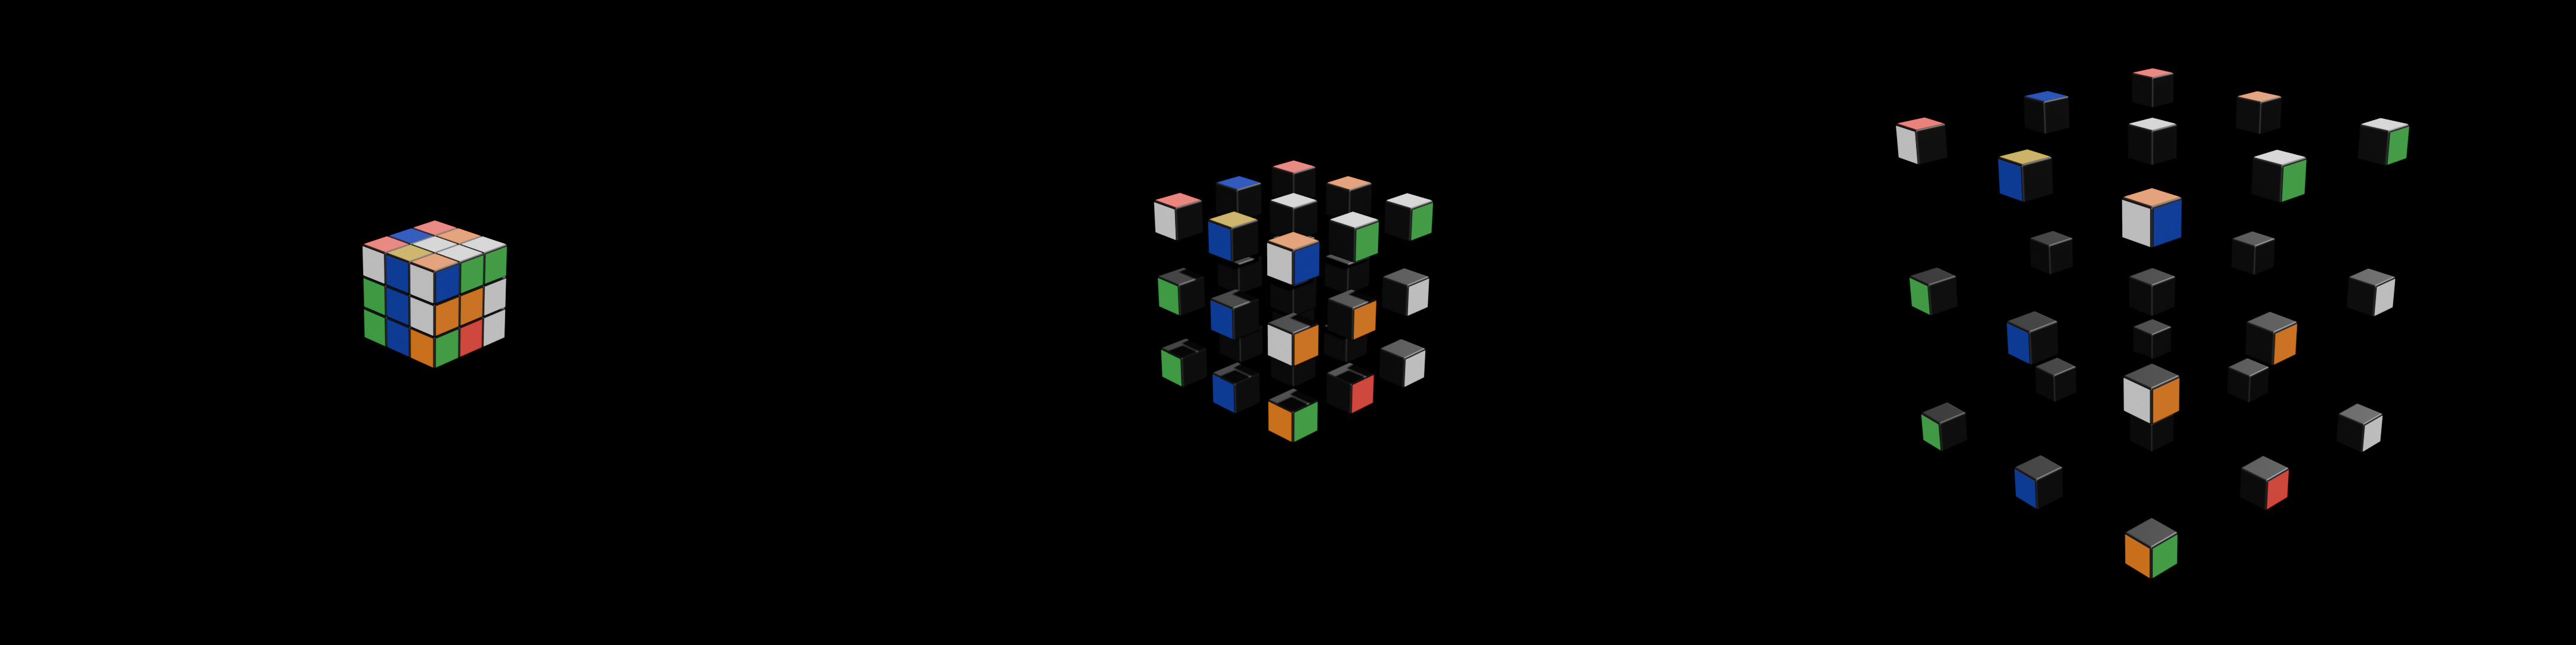
\includegraphics[width=1\textwidth]{images/RubiksExplosion.png}
    \caption{Beispiel einer Explosionsanimation anhand eines Rubiks Cube}
    \label{fig:rubiks-explosion}
\end{figure}

Die Requirements sollen in Form von Text auf UI-Panels dargestellt werden, welche an den zugehörigen Bauteilen angebracht sind.


Bei komplexen Produkten mit einer Vielzahl an Bauteilen, wie beispielsweise einem Fahrzeug, existiert eine hohe Anzahl an Requirements.
Eine gleichzeitige Animation aller Komponenten würde dann bei komplexen Produkten zu einer übermäßigen Zahl an Requirements führen, die gleichzeitig dargestellt werden müssten.
Daher ist es bei umfangreichen Produkten eventuell sinnvoll, die Darstellung der Bauteile in mehreren Schritten zu realisieren.
Dafür könnten Bauteile des Produkts, die aus mehreren anderen Bauteilen bestehen, als separate Produkte mit ihrer eigenen Explosionsanimation betrachtet werden.
Ein Beispiel für eine Komplettübersicht ist die Darstellung eines kompletten Fahrzeugs in wenigen Bauteilen.
Dabei wird ein Rad, das aus Reifen, Felge, Radmuttern, Bremsscheibe etc. besteht, als ein einzelnes zusammengehöriges Objekt behandelt.
Bei Bedarf kann der Nutzer in eine Detailansicht wechseln, in der lediglich ein Rad mit all seinen Bauteilen animiert wird.
Durch eine Verschachtelung von immer detaillierteren Ansichten kann eine hohe Komplexität der Darstellung erreicht werden, ohne dass die Übersichtlichkeit durch eine zu hohe Anzahl an Requirements gleichzeitig verloren geht.
Dieses Prinzip der Verschachtelung ist auch im Ablaufdiagramm in Abbildung \ref{fig:explosions-ablauf} anhand der beiden rechts und links abgehenden Schleifen des unteren Entscheidungsblocks zu erkennen.

\begin{figure}[H]
  \centering
  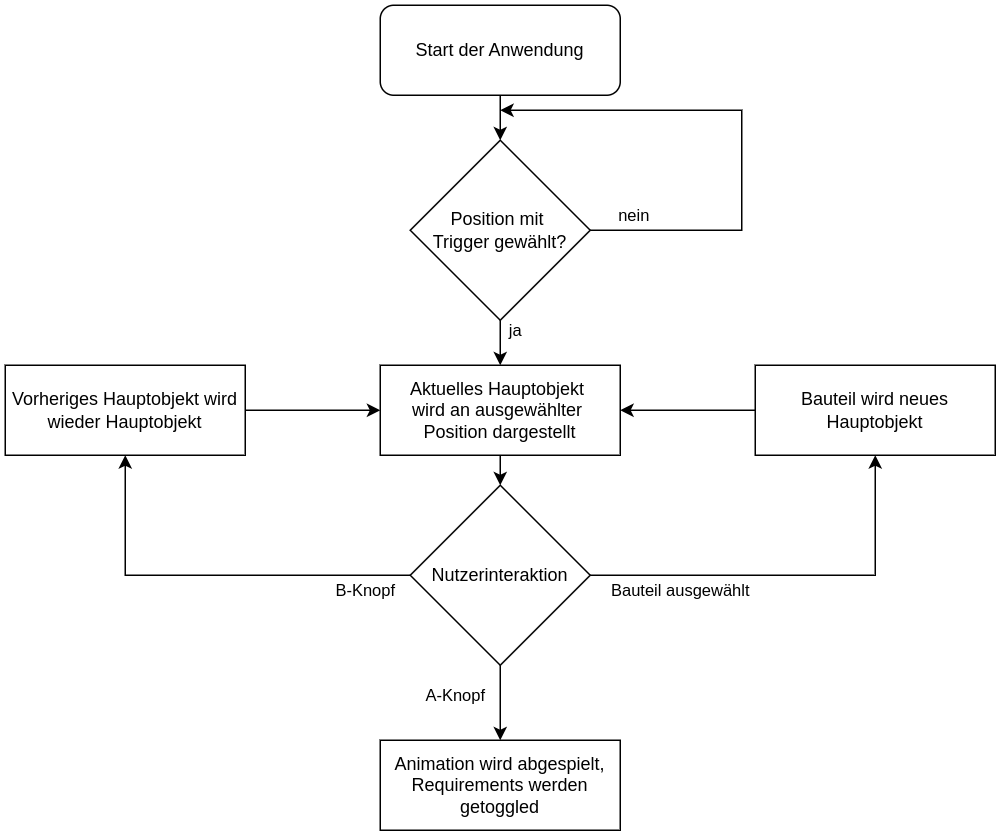
\includegraphics[width=0.8\textwidth]{images/ExplosionAblauf.png}
  \caption{Ablaufdiagramm des Interaktionskonzepts der Explodierenden Bauteile}
  \label{fig:explosions-ablauf}
\end{figure}

Für diese Darstellung soll der Nutzer, wie am ersten Entscheidungsblock im Diagramm in Abbildung \ref{fig:explosions-ablauf} zu sehen ist, zunächst mithilfe eines Controllers einen Ort für die Darstellung im Raum auswählen.
Der ausgewählte Punkt im Raum wird als Ursprungspunkt für die Darstellung der Bauteile verwendet.
Anschließend hat der Nutzer die Möglichkeit, die Explosionsanimation des aktuell angezeigten Modells per Knopfdruck zu aktivieren.
Beim Drücken des A-Knopfs wird dann die Animation des aktuellen 3D-Modells abgespielt und den Bauteilen werden ihre Requirement-Panels angehängt.

Alternativ besteht für den Anwender die Möglichkeit, mit dem Trigger ein anderes Bauteil auszuwählen, um dieses als neues Hauptmodell anzuzeigen und somit dessen Requirements zu betrachten.
Durch Betätigen des B-Knopfes erfolgt eine Reduzierung des Detailgrads der Darstellung, sodass die vorherige Ansicht wiedergegeben wird.

Auch bei Software-Requirements ist es denkbar, diese in ihre Komponenten zu zerlegen und zu diesen Komponenten zugehörige Requirements darzustellen.
Jedoch bietet die Darstellung in AR bzw. VR hierbei quasi keine Vorteile im Gegensatz zu einer 2D-Darstellung auf einem Bildschirm.
Bei Software-Anwendungen ist die einfache Darstellung auf einem Bildschirm näher an der tatsächlichen Laufumgebung der meisten Softwareprodukte weshalb das Konzept eher für physische Produkte sinnvoll ist.

Bereits bei der Erstellung des Konzepts wird ersichtlich, dass einige der Implementierungsschritte, wie beispielsweise das Erstellen der Animation, einen hohen Zeitaufwand erfordern können.
Im Rahmen dieses Interaktionskonzepts soll daher die Realisierbarkeit solcher Darstellungen für physische Produkte untersucht werden.
In diesem Zusammenhang ist zu berücksichtigen, dass aufgrund des zu erwartenden hohen Zeitaufwands für die Implementierung eine kritische Betrachtung der Kosten-Nutzen-Relation erforderlich ist.
Um dennoch eine sinnvolle Grundlage für die tatsächliche Anwendung zu bieten, muss das Interaktionskonzept einen wesentlichen Mehrwert bei der Vermittlung der Requirements aufweisen.
%DeepL korrigiert

\newpage
\section{Wolken von Requirements}

Der Ansatz der explodierenden Bauteile ist aufgrund der individuellen Ausgestaltung des Interaktionskonzepts mit einem hohen Zeitaufwand und einer komplexen Umsetzung verbunden.
Des Weiteren ist zu berücksichtigen, dass dieser Ansatz lediglich für die Darstellung von Produkten, also physischen Systemen, geeignet ist.
Daher wird ein weiteres Interaktionskonzept entwickelt, welches sich theoretisch auch automatisiert generieren lassen soll und für alle Arten von Requirements geeignet ist.

Des Weiteren ist beabsichtigt, eine Übersicht über eine größere Anzahl von Requirements gleichzeitig zu erlangen, als im ersten Interaktionskonzept möglich war.
Dadurch soll eine visuelle Darstellung vieler Requirements gleichzeitig ermöglicht werden.

Die grundlegende Idee ist, Requirements in Wolken von Texten darzustellen, also als wolkenförmige Gruppierungen von UI-Elementen im Raum.
Die UI-Elemente sollen dabei Panels sein, auf denen der Text der Requirements sowie weiterführende Informationen zu den Requirements dargestellt werden.
Diese Panels sollen dann in einer Wolkenartigen Anrichtung, ähnlich wie die Punktewolke in Abbildung \ref{fig:point-cloud}, dargestellt werden.

%DeepL korrigiert

\begin{figure}[H]
    \centering
    \includegraphics[width=0.6\textwidth]{images/PointCloud.jpg}
    \caption{Beispiel einer Punktewolke}
    \source{\autocite{PointCloud}}
    \label{fig:point-cloud}
  \end{figure}



Im Rahmen dessen soll eine räumliche Gruppierung der Requirements nach verschiedenen Kriterien ermöglicht werden.
So wäre es beispielsweise denkbar, Requirements, die zu einem bestimmten Feature gehören, in einer Wolke zu gruppieren, während Requirements, die zu einem anderen Feature gehören, in einer anderen Wolke gruppiert werden.
Die räumliche Anordnung der Wolken soll es dem Nutzer ermöglichen, schnell zu erkennen, welche Requirements nach der aktuellen Filterung eine hohe Korrelation aufweisen und welche nicht.

Des Weiteren ist vorgesehen, dass eine Zoomfunktion implementiert wird, mittels derer es möglich ist, in die Wolke hinein- und herauszuzoomen, um die Granularität der angezeigten Requirements zu erhöhen.
Ein Beispiel für eine mögliche Umsetzung wäre, dass in großen Wolken initial nur Punkte als Repräsentationen von Requirements angezeigt werden, in welche man hereinzoomen kann, um die Requirements zu lesen.
In einem nächsten Schritt besteht die Option, wieder heraus zu zoomen und somit wieder eine Übersicht über eine größere Anzahl an Requirements der Wolke zu erlangen.

Eine weitere Möglichkeit wäre die Implementierung von Filtermöglichkeiten für verschiedene Beziehungen des Requirements auf den Requirementspanels, sodass bei einer Auswahl in die neue Requirementswolke gewechselt werden kann.
Die Interaktion sowie die räumliche Anordnung der Wolken zielen darauf ab, dem Nutzer auch bei einer großen Anzahl von Requirements einen Überblick zu gewährleisten und eine schnelle Auffindbarkeit der gewünschten Requirements zu ermöglichen.

Bei diesem Konzept soll insbesondere der Vorteil gegenüber einer zweidimensionalen Darstellung kritisch analysiert werden.
Denn die Darstellung der Requirements in Wolken ist prinzipiell auch in 2D möglich, auch mit der Interaktionsmöglichkeit des Hinein- und Herauszoomens.
In diesem Zusammenhang ist zu untersuchen, ob die räumliche Anordnung der Requirements in AR tatsächlich einen Mehrwert gegenüber einer 2D-Darstellung bietet und ob die Interaktionen intuitiv und effizient sind.
Zudem soll ein Fokus darauf liegen, auch große Zahlen von Requirements gleichzeitig darzustellen.

%DeepL korrigiert